\chapter{Theory}
\label{theory}

From meetings with the municipality and the Norwegian Public Roads Administration, and the pre-project leading up to this thesis, much of the background theory has come to light. Here the material is going to be presented. First in a section that covers theory on winter road maintenance. Then in the rest of the chapter focus will be on routing problems, and how the theory can be applied to the situation in Trondheim.

\section{Winter Road Maintenance} % (fold)
\label{sec:snow_plowing}

% \begin{wrapfigure}{o}{0.5\textwidth}
%     \begin{center}
%         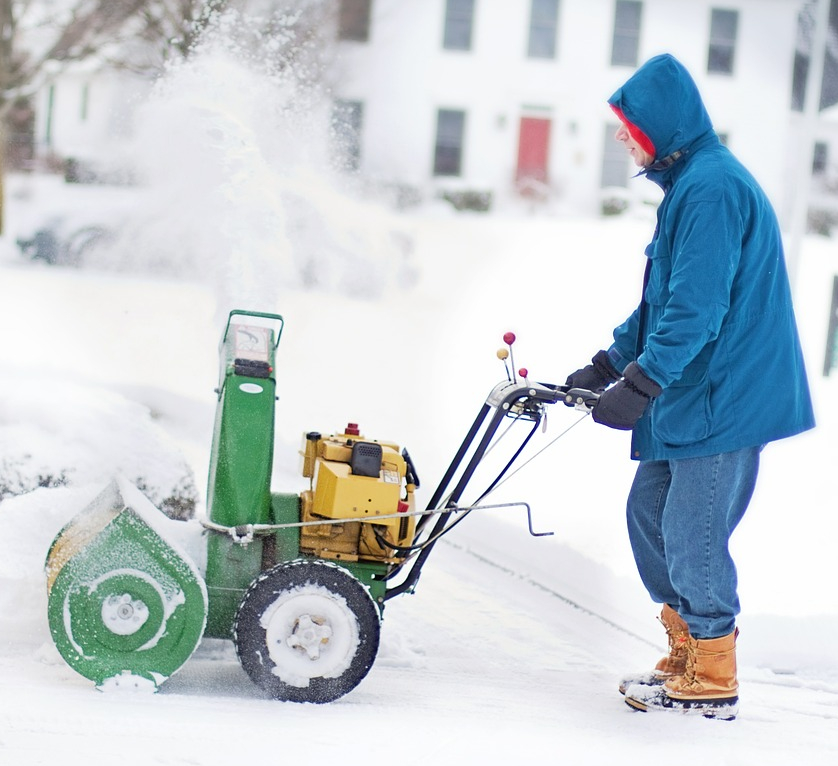
\includegraphics[width=0.5\textwidth]{figures/MachineryIllustrations/pixabay_snow-blower-584380_1280.jpg}
%     \end{center}
%     \caption{Snowblower}
%     \label{fig:snowblower}
%     % source (2015-06-03T23:38:30Z): http://pixabay.com/en/snow-blower-man-work-winter-snow-584380/
%     % license: CC0
% \end{wrapfigure}

\begin{wrapfigure}{o}{0.5\textwidth}
    \begin{center}
        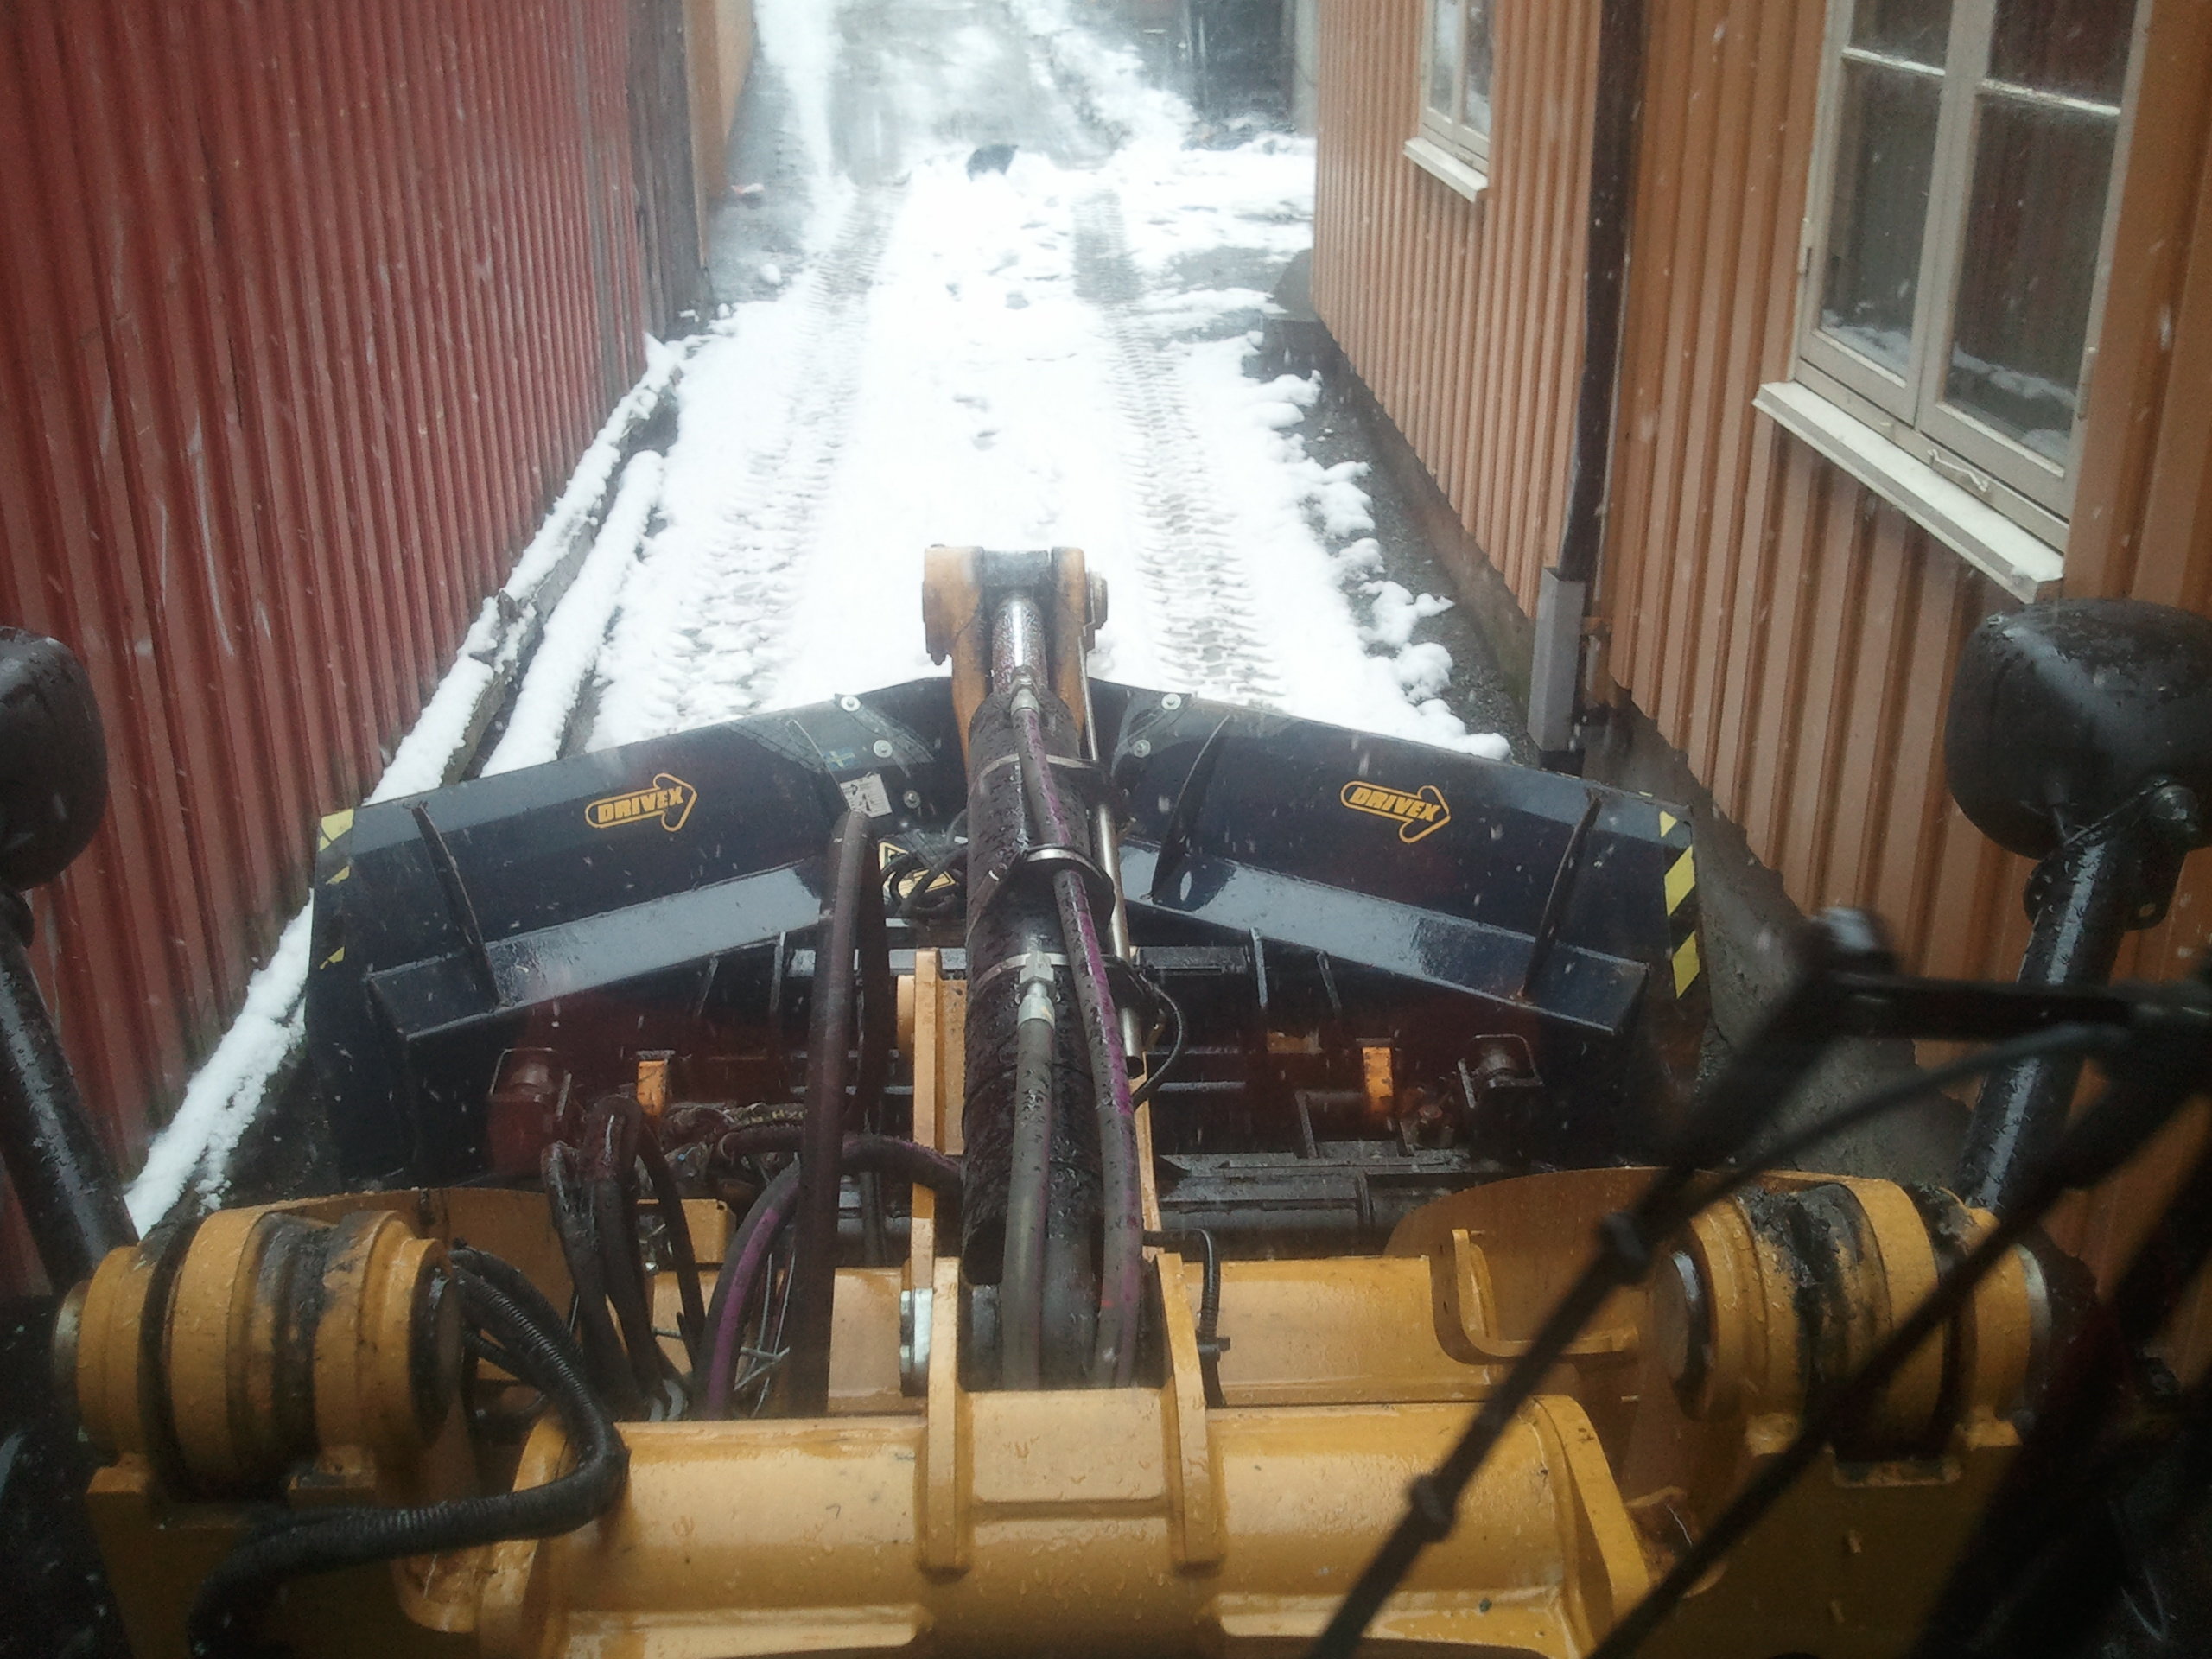
\includegraphics[width=0.5\textwidth]{figures/MachineryIllustrations/snowplow-Kent_Syrstadlokk-2012-04-18.jpg}
    \end{center}
    \caption{Snowplow in a Trondheim alley. Copyright Kent Syrstadløkk 2015, with permission.}
    \label{fig:snowplow_in_alley}
\end{wrapfigure}

In places where the temperature regularly goes below the freezing point of water, winter road maintenance has to be performed. Under such conditions, ice can grow on the roads, and they might become blocked by snow. The work done in ensuring that the roads have enough friction to be safe for use by pedestrians and vehicles, and clear enough of snow so that they may pass at all, is what is called winter road maintenance.

The three most common ways of performing winter road maintenance are gritting, salting, and plowing. Gritting describes the act of spreading granular materials, such as pebbles or sand, on slippery surfaces so that they get more friction. It is often performed on walkways and smaller roads as less resource intensive way to temporarily make it safe for pedestrians and roads with light traffic. In practice, sand and combinations of sand and salt are preferred over pebbles when gritting.

Salting is similar to gritting in the sense that the same vehicles and rudimentary process is used to distribute it. However it acts in a different way, and there are other constraints to consider when using it. As opposed to gritting, salting is not done to increase the friction on top of the snow or ice that may be on the road. Instead, it is done to melt ice, or ensure that ice does not form in the first place. Thus, a desired amount of friction is achieved by keeping the road clean. The main challenge with salting and the reason that gritting may be preferred over salting in many situations is that salting on top of a layer of snow has disastrous results. One gets a slippery, gooey matter that cannot easily be removed from the road other than by scraping it off. Therefore, it is almost always performed as a preventative measure, usually right after a stretch of road has been plowed.

Snow plowing is when snow is cleared by pushing it aside. In daily life, various tools are used for clearing snow in this way, such as for an instance general purpose or specialized snow shovels. However, for road maintenance vehicle mounted snowplows are the preferred appliance. Although they are not suitable for improving friction arising due to ice, snowplows are great at handling snow that is a direct obstacle to the traffic. Also, they can improve the friction by removing densely packed and polished tracks in the snow.

\subsection{Organization of Winter Road Maintenance in Norway and Trondheim} % (fold)
\label{ssub:how_winter_road_maintenance_is_organized_in_norway_and_trondheim}


In Norway, the winter road maintenance is a responsibility that is divided between the NPRA, the local municipalities, and the owners of private roads (which are responsible for maintaining their own roads). The NPRA has issued a handbook, R610 \citep{svvR610}, which specifies the constraints on when what kind of winter road maintenance should be performed, and what condition roads should be in after they have been serviced. In the handbook, they define five classes of winter maintenance standards for roads, as shown in Table \ref{tab:wmscfrsbtn}.

\rowcolors{2}{gray!15}{white}
\begin{table}[tbph]
\centering
%ref page 120 in http://www.vegvesen.no/_attachment/61430/binary/964067?fast_title=H%C3%A5ndbok+R610+Standard+for+drift+og+vedlikehold+av+riksveger.pdf
\resizebox{\textwidth}{!}{
\begin{tabular}{l p{0.55\textwidth}} % {0.38\textwidth} {0.62\textwidth}
\hline
\textbf{Class Name}                 &  \textbf{Class Description}                                                                                    \\ \hline
Winter maintenance class A -- DkA  &  Approved road condition is bare road (dry or wet).                                                                                  \\
Winter maintenance class B -- DkB  &   Approved road condition is bare road (dry or wet),  hard snow/ice is permissible outside rut\footnotemark for limited periods.                    \\
Winter maintenance class C -- DkC  &  Approved road condition is bare road (dry or wet) in mild periods and hard snow/ice in cold periods.                                \\
Winter maintenance class D -- DkD  &  Approved road condition is hard snow/ice.                                                                                           \\
Winter maintenance class E -- DkE  &  Approved road condition is hard snow/ice.  Friction as low as 0.20 is acceptable. DkE may not be used for national roads.  \\ \hline
\end{tabular}
}
\caption{Winter maintenance standard classes for roads specified by the NPRA (author's translation)}
\label{tab:wmscfrsbtn}
\end{table}
\footnotetext{track in the road made by the wheels when many vehicles often pass }

Besides being sorted into one of these maintenance classes, each road is also sorted into a functional class by the NPRA. In total, the NPRA operates with ten functional classes depending on factors such as the amount of daily traffic or size. However, Trondheim municipality only operates with six functional classes of roads in their maps. They are shown in the list below as translated by the author, and an example can be seen in Figure \ref{fig:map_KV_B_used}. Because the text will mainly be considering winter road maintenance from the municipality's perspective, those are the definitions that will be used further in this text.

\begin{landscape}
\begin{figure}[thbp]
    \centerline{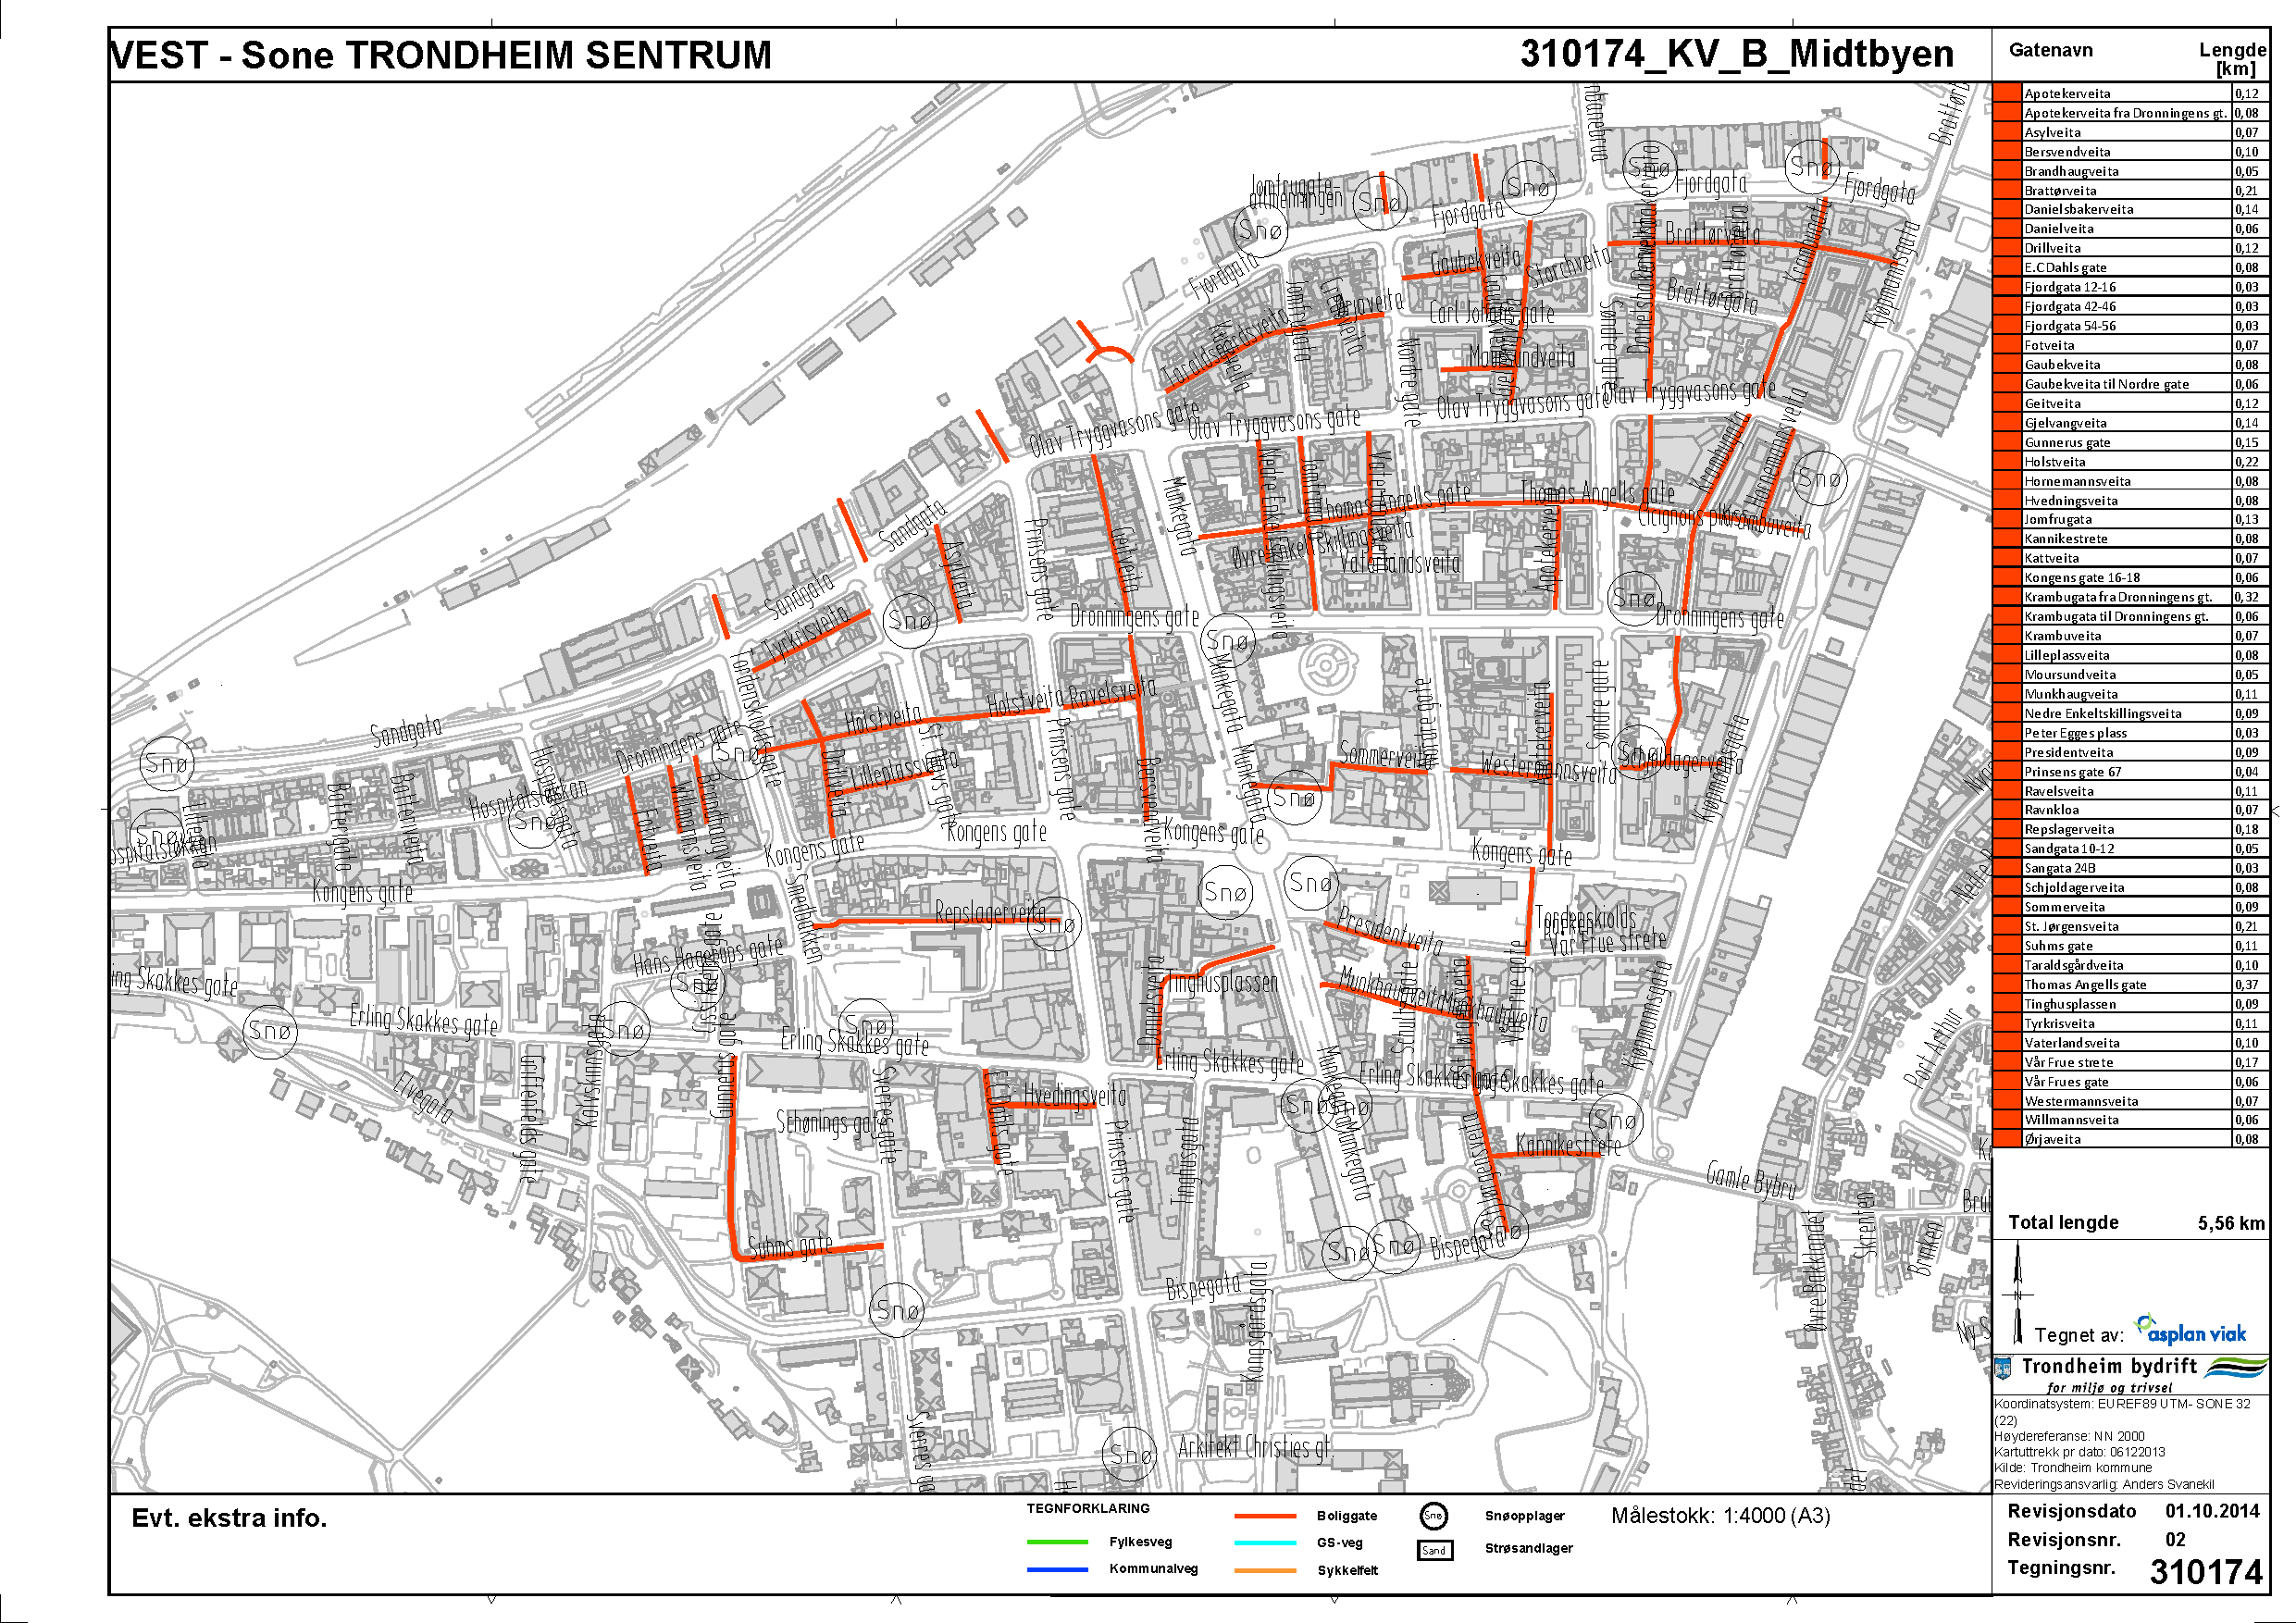
\includegraphics[height=0.945\textwidth]{figures/Routes/PreExisting/310174.pdf}}
    \caption{Map of a route driven in Trondheim. Copyright Trondheim Kommune 2015, with permission.}
    \label{fig:map_KV_B_used}
\end{figure}
\end{landscape}

\begin{itemize}
    \item Riksveg (National road)
    \item Fylkesveg (County road)
    \item Kommunalveg/Hovedveg (Municipal road)
    \item Boliggate (Street)
    \item GS-veg (abbreviation for Gang- og Sykkelvei, translates to Footpaths and Cycle Paths) %https://www.regjeringen.no/en/topics/municipalities-and-regions/by--og-stedsutvikling/framtidensbyer/area-and-transport/footpaths-and-cycle-paths/id547994/
    \item Sykkelfelt (Bicycle lane/path)
\end{itemize}


Out of these, the municipality is responsible is responsible for maintaining all, except national and county roads, for which the responsibility falls to the NPRA. As of February the 25th 2015, there are 212 km of municipal roads, 336 km of streets, and 180 km of footpaths and cycle paths that the municipality of Trondheim is responsible for maintaining during the winter (\citep{trondheimKommuneVinterdriftNettside}, only in Norwegian). To make servicing all these 728 km of roads feasible, they have divided the road network into several smaller zones.

An important factor in deciding the zones is what amount of work can be performed in one trip with the equipment. For gritting, the size of each zone may depend on how much sand can be carried before the vehicle has to return to a sand depot to refill. When plowing, the size of the zone might be restricted by how fast a vehicle can cover the entirety of it so that it is returned to the required condition before too much time has passed.

Another important thing that has been considered when creating the zones is what type of equipment is suitable for processing what kind of road. The large municipal roads might be suitable to service with a snowplow truck. Smaller alleys and streets, on the other hand, are better approached with smaller tractors that can fit through them. Therefore when looking at the zones it can be seen that many of them are inside the same area of the map, but containing different roads.

Something the zones in overlapping areas of the map do have in common are the places where the snow is to be stored and disposed of. In the countryside, the snow can often be dumped on the side of the road and left there. However, in cities, and densely populated areas, it is not so simple. There are various snow depots where the snow is moved for long-term storage, and the snow that gets cleared from the city centers proximity is put into the ocean at the harbor. However, all of the snow cannot be immediately moved to these locations while the roads are being cleared. Therefore, as can be seen on the municipality's maps, there are marked several areas where snow can be temporarily stored while the work is being performed.

To complete all of this work, the municipality has chosen to handle some of the zones themselves, and set out the other to contractors. The municipality has a lot of the equipment needed for handling the biggest roads, and the intricate situation in the city center. To operate their equipment they use their own drivers. The contractors handling the remaining roads range from individuals that use their own vehicles (typically tractors), to specialized companies with several vehicles and drivers. All of the work is coordinated centrally, by the management at the municipality. They organize both the work carried out by the municipality's drivers, and that done by the contractors. They set up the schedules for the maintenance work that needs to be done regularly and call out individual drivers when there has been a weather-incident.

% subsubsection how_winter_road_maintenance_is_organized_in_norway_and_trondheim (end)

Given this outline of how the municipality handles the snow removal part of winter road maintenance, how snow plowing can be modelled and solved needs to be addressed. The next section will explore the models used for similar problems to routing for snow plowing, and what methods have been used to try to find solutions to them.

% section snow_plowing (end)

\section{The Node, Edge, and Arc Routing Problem}
\label{the_nearp}

In the pre-project leading up to this thesis, a structured literature review was performed \citep{forprosjektet}. The focus was finding whether routing for snow plowing as in Trondheim is a known and solved problem. Moreover, in case it is, how should one go about trying to solve it.

In the structured literature review, it was found that the current take on problems like snow plowing has long roots. The simplest possible interpretation is that it is about traversing a graph G=\{N,E\} in a certain way. Which would make it similar to the “Seven Bridges of Königsberg Problem”, that is about finding a cycle that traverses the graph and visits all the edges exactly once, and was solved by the Swiss mathematician Leonhard Euler in 1735 \citep{eulerBridges}.

However, it was not until more than 200 years later (in 1962) that a graph traversal problem that is more relevant to snow plowing was proposed \citep{wohlk2008decade}. The Chinese mathematician and former postman, Mei-Ko Kwan described the problem of finding the shortest trip that visits all the edges in a graph at least once \citep{meiKoKwanCPP}. It is the converse of the Vehicle Routing Problem (VRP), which is about visiting all the nodes of the graph at the lowest possible cost \citep{laporte1992vehicle}. The problem became known as the Chinese Postman Problem (CPP).

The CPP, if it contains only undirected edges or directed edges (arcs) (G=\{N,E\} or G=\{N,A\}), can be solved in polynomial time \citep{wohlk2008decade}. But if it is a mixed graph containing both (G=\{N,E,A\}) it is NP-hard \citep{wohlk2008decade}.

Over the following decades, several variations on the problem were made to handle specific challenges. Here follow definitions of some of the most known formulations and how they are tied to snow plowing:

\begin{description}

\item [The Rural Postman Problem (RPP)] arose when one wanted to optimize solutions for when the postman does not have to visit all the edges, but only a subset of them \citep{pearn1995RPP}. That is a situation that is likely to arise in snow plowing, where one for an instance has to service all the roads in a city with a certain amount of traffic. In such a scenario, one can pass through the less used roads to move between the ones that have to be plowed.



\item [The Mixed Chinese Postman Problem (MCPP)] is the approach to the CPP where one looks at the problem in a mixed graph (with both arcs and edges) \citep{pearn1995mixedCPP}. It introduces a relevant constraint when considering practical applications, such as snow plowing, where the underlying graph represents a road network. Not only is it a very natural representation of a road network containing both bi-directional and one-way roads, it can also be used to handle cases such as intersections with forbidden turns.

\item [The Hierarchical Chinese Postman Problem (HCPP)] \citep{ghiani2000HCPP} came about when one wanted to investigate how solutions would change if one required some edges to be serviced before others. It is a situation that often arises in practice. For an instance in snow plowing one might want to service a more used road before a less used road.

\item [The Windy Postman Problem (WPP)] is the attempt at accounting for that an edge can have a different cost each time you pass through it \citep{dussault2013WPP}. This is a relevant consideration when snow plowing, because simply passing through a road and plowing it takes a different amount of resources and time. Even passing through a road that has already been plowed and one that has not can have separate costs.

\item [The k-postman Chinese Postman Problem (k-CPP)] is the attempt at modeling a scenario where there is a depot node, and k postmen \citep{edmonds1973kCPP}. It can also be interpreted as one postman that can do k trips of a certain cost. If implemented correctly it can be argued that splitted trips from the k-CPP can be used for sectoring the road network between different contractors.

\item[The Min-Max k-CPP (MM k-CPP)] takes it a step further and looks at minimizing the trip with the maximal cost of the k trips \citep{frederickson1976MMkCPP}. It is relevant for the snow plowing case when there is a large road network, and there is no single vehicle that is capable of service all of it in one go. 

\end{description}

All these variations on the CPP are focused on general graphs, although they arguably can be applied to a broad spectrum of tasks in real-world road networks. However the Arc Routing Problem (ARP) has in the meantime been defined to describe problems centered around servicing arcs in transport networks \citep{eiselt1995ARP}. The main difference from the various CPPs tends to be the more vehicle oriented terminology that is used, which makes it somewhat difficult to describe how they relate to one another. It can both be argued that the ARP is a more general version of the CPP with a slightly different terminology, or that it is a special applied case of the CPP.

In later years, the literature dealing with applied routing with the goal of visiting/servicing the arcs and/or edges in a graph has been favoring the ARPs terminology over that of the CPP. This widespread use makes it an interesting approach to the issue of routing for snow plowing.

Especially the variation known as the Capacitated Arc Routing Problem (CARP) \citep{ulusoy1985CARP} has been widely studied. It has much in common with the k-CPP, because it deals with the case of having a set of identical vehicles with a limited capacity located at a depot. The task of which is to service the roads in a network in such a way that each road gets serviced by one vehicle once. However, like the k-CPP it suffers from that it is too general to give a good description of complex problems like snow plowing.

This lack of clarity has in turn given rise to definitions that try to include more constraints so that the problems one wants to solve are more accurately described. Within the ARP paradigm, the Extended Capacitated Arc Routing Problem (ECARP) has been defined to handle this \citep{lacomme2004competitiveMA}. It tries to take into account things such as that the problem might be in a mixed graph, the edges/arcs can have a varying cost, special constraints such as u-turns being forbidden in ordinary intersections, or a maximum limit on trip lengths.

The problem definition found that fits the case of Trondheim best, however, is the Node Edge and Arc Routing Problem (NEARP) \citep{prins2005memeticNEARP}. It describes the problem of servicing a subset of the nodes, edges, and arcs in a mixed graph, with a homogeneous set of vehicles. Like in the k-CPP and CARP, each vehicle is capacitated in terms of demand it can service (cost it can handle). The elements of the graph that require servicing have a fixed demand, and all of the arcs and edges have a traversal cost while nodes have no traversal cost (although required nodes do have a servicing cost).

Because it combines the CARP, VRP, and the General Routing Problem, it takes into account many of the features of the underlying network desired to use for structuring the graph, such as the assumption of a mixed graph. Another feature that makes it a better model is that it considers both nodes, arcs, and edges as elements of the graph that can need servicing. This assumption makes sense in a snow plowing setting, where not only roads and one-way roads, but also intersections need to be plowed.

Now with the definition of what kind of problem snow plowing in Trondheim having been presented, how it can be solved should be considered.


% section the_nearp (end)

% Historical approaches and solutions -> What we gonna use ((M)EA) -> EA -> Fitness -> FLW (basiskomponent) -> Grand tour vs Split som fitness -> Split forklart.

\section{Routing Algorithm's} % (fold)
\label{sec:routing_algorithms}

In the structured literature review, several methods of solving routing problems came to light. Clearly, the most desirable outcome would be a solution that is known to be optimal. Moreover, for the polynomial time cases such as the plain CPP where all the edges have to be serviced by one postman, exact solutions methods exist. However, for the NP-hard cases like the CARP, exact solutions quickly become infeasible as problem sizes grow. Some of the best exact approaches have been reported to perform well for problems with up to 7 vehicles, 50 nodes, and 97 edges \citep{belenguer2003cutting}.

These limitations of the exact methods have lead to efforts in pursuing other ways of finding solutions. Some have tried probabilistic approaches \citep{christiansen2009branch}, but the majority of work has been done on heuristic methods. Simulated Annealing \citep{eglese1994simulatedAnnealing} and Tabu search \citep{brandao2008tabu} have been used successfully to give good results. It has also been shown that A* can give approximate solutions \citep{rao2011AStar}. However, this approach suffers from that there is a significant tradeoff between the quality of the solutions it finds and its capability of processing larger problems within reasonable time.

Other methods that have shown to be robust both in terms of quality of solutions are Ant Colony Optimization (ACO) \citep{santos2010ACO} and Greedy Randomized Adaptive Search Procedure (GRASP) \citep{usberti2013grasp}. Both yield solutions of similar quality to those found by Tabu Search, but ACO outperforms GRASP on running time.

Lately, the most promising results have been given by Evolutionary Algorithm's (EA's). GA's, a common type of EA's, have been shown to provide high-quality solutions for large instances of the CARP/NEARP \citep{lacomme2001GA}, and generally to outperform other non-evolutionary methods \citep{wohlk2008decade}. A further improvement on GA's has been made by MA's \citep{prins2005memeticNEARP}. They have a reasonable running time, and they are capable of finding the highest quality solutions for the larger problem instances.

As such MAs can be considered as the current state of the art approach to solving NEARPs, which is the reason they have been chosen for the work with snow plowing in Trondheim in this thesis.

% section routing_algorithms (end)


\section{Evolutionary Algorithm's} % (fold)
\label{sec:evolutionary_algorithms}
Now that the reasons for using an EA has been laid out, what EA's are, and how they can be implemented should be discussed. EA's were one of the earliest bio-inspired algorithm's, whose outline were first discussed by Alan Turing in \citet{turing1950computing}. The idea is that EA's should mimic the biological processes in evolution, abstracting potential solutions to a population of individuals that have traits that are combined and altered through generations.


\begin{wrapfigure}{o}{0.4\textwidth}
    \begin{center}
        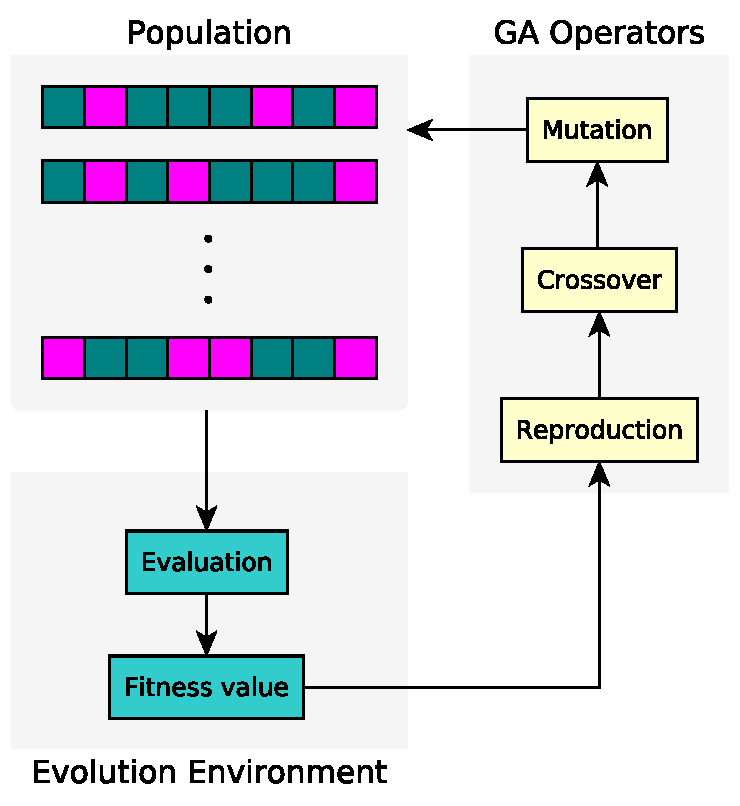
\includegraphics[width=0.4\textwidth]{figures/GA_general_flow_illustration.pdf}
    \end{center}
    \caption{How evolution flows in genetic algorithm's. Reproduced according illustraion in \citet{gaFlowIllustrationSource}}
    \label{fig:ga_flow_illustraion}
\end{wrapfigure}


A common variant of EA's are GA's, as presented in \citet{holland1975originalGA}. An illustration of their general workflow can be found in Figure \ref{fig:ga_flow_illustraion}. In the paradigm of the GA, at the core of each individual there is a genome. This genome is an alternative representation of a solution to the problem one is trying to solve with the GA, which satisfies certain properties.

When there is a new generation, new individuals are made by combining existing members of the population. This combination is done by taking two or more individuals and combining their genomes into a new genome, which becomes the foundation for a new individual. This process is often called crossover. A genome must thus be constructed so that it can be merged with another genome in such a way that the output is a valid genome that represents a solution.

Each new genome, when created, has a chance of undergoing mutation. In practice, this often means that one of its components gets an altered value, or two components swap places in the genome, yielding a new altered genome. What this does is that it ensures that there is always some random variation in the population, making it less prone to becoming stuck in a local optimum.

It must also be possible to convert a genome to a solution of the problem the GA is trying to solve. The solution obtained from a genome is called an individual's phenotype. These phenotypes should take a reasonable time to generate, especially because they are often the foundation for calculating an individual's fitness.

The fitness can then be used to determine whether an optimal solution to the problem has been found. If not, for an instance because it is unknown what a problems global optimal value is, the fitness is often used in determining what individuals are coupled when the nex generation is created. It is also utilized to find what combination of pre-existing individuals and new individuals should make up the population at the end of the generation/beginning of the next generation.

To improve on GA's the concept of memetics can be introduced, turning them into MAs \citep{moscato1989memeticism}. Memetics is the term used for describing that individuals can be improved after being generated, mimicking the ability of real life organism in evolutionary systems to learn. In practice, this is often done by replacing the mutation step with doing a simple local search, such as hill climbing, to improve the genome \citep{lacomme2004competitiveMA}.

With the genome being such a central piece in making an EA work, it is natural to let it be the first thing one considers when making a specialized EA for an instance for snow plowing. Initially, the approach was to figure out what the genome was to represent. In the case of routing for snow plowing, a solution, and thus what the genome should represent is a route for a snow plow. However, what if there, like in the k-CPP and CARP, are several snow plows? Then the genome has to represent a set of trips for each vehicle. Ideally, the genome should be able to represent both these cases.

The solution found in the literature was to let the genome represent a single circular route, a grand tour of the underlying graph as done in \citet{lacomme2001GA}. When dealing with multiple vehicles this tour is splitted into several shorter trips, one for each vehicle. Once the genome and the phenotype it represents is decided, one can begin to look into how the goodness of each individual should be determined, ie. how to calculate the fitness.

% Circular, splittable. 
% Underlying graph -> graph as set -> required elements.
% Giant trip and splittable

% Snow plowing -> Snow plowing genome / phenotype -> How to fitness.

\subsection{Fitness for Snow Plowing} % (fold)
\label{sub:fitness_for_snow_plowing}

There are many things to keep in mind when trying to determine the fitness of a route in a complex operation like snow plowing. In interviews with the municipality and the NPRA, some of the most important factors that impact the execution of the plowing, and most likely should affect the goodness of a solution were discussed.\footnote{Meeting with Trondheim Municipality and the NPRA. Trondheim Bydrift, 3. etage, Tempeveien 22, 7031 Trondheim, Norway. 2014-09-02 09:00.} They are shown in figures \ref{fig:environmental_factors} and \ref{fig:imposed_constraints}.


\begin{figure}[thbp]
\caption{Factors arising from the environment}
\label{fig:environmental_factors}
\begin{description}[noitemsep,nolistsep]
    \item [Amount of traffic.] If there is much traffic, the plows should be expected to move slower.
    \item [Obstacles such as barriers and curbstones.] Some barriers are designed so that they can be forced by sturdy vehicles such as snow plows moving slowly while other barriers cannot be passed. Other obstacles such as curbstones can be driven over by some vehicles while others would be stopped or would damage the curbstone in passing over it.
    \item [Road marking and regulation.] Some places snow plows could be exempt in the marking, allowing them to pass through and service roads other traffic would normally not be permitted to access. Road markings such as forbidden turns should also be taken into consideration when making and working on the graph based on the underlying road network.
    \item [Slope of the road.] The slope of the road influences how quickly it can be worked on, and in some instances what type of equipment is suitable for the job (for an instance whether tire chains have to be used).
    \item [Speed limit.] The speed limit will determine how fast a road can be worked on, how suitable it is for accessing other parts of the road network, as well as its traffic pattern.
    \item [Weather -- Quality of the snow.] A lot of wet, heavy, and dense snow will require the vehicles to use more power than a dry, light, and powdery snow.
    \item [Weather -- Slipperiness of the road.] If there is much ice and the road is very slippery the vehicles can be expected to work slower.
    \item [Width of the road.] Affects whether it can be done by a single vehicle in one pass or not, and what kind of vehicle is suitable.
\end{description}
\end{figure}

\begin{figure}[thbp]
\caption{Constraints on how the work should be carried out}
\label{fig:imposed_constraints}
\begin{description}[noitemsep,nolistsep]
    \item [Equipment -- Amount of vehicles available.] If there are more vehicles available they can split the road network between each other and the work can be carried out and completed faster.
    \item [Equipment -- Types of vehicles available.] Not all vehicles are suitable for plowing all roads. The larger vehicles used for plowing the main streets cannot enter and plow narrow alleys. Conversely, the vehicles used for plowing alleys or pavements would be inefficient at clearing wider roads.
    % \item [The order in which the roads are serviced.] 
    \item [The weather.] The NPRA has specified when maintenance should be done \citep{svvR610}, and what shape the road should be in after the maintenance is done.
    \item [The type of road.] Some roads have higher priorities than other roads.
    \item [Where the snow can be stored.] Snow cannot always just be showed to the side out of the road. At times, there will be sidewalks or bicycle paths there that should not be blocked by the operation just to have to be services again later. There are pre-defined areas where the snow can be deposited.
\end{description}
\end{figure}

% When what is needed to calculate the fitness has been obtained, the next step becomes setting up the calculation process.

When one has gained an overview of what variables are required to find the fitness, the next task becomes setting up the calculation. The format of the benchmarks that have been chosen as the input format dictates how the values are supplied to the algorithm. Each edge and arc has an associated cost of passing through without doing work, the deadheading cost. Nodes have no deadheading cost. All the factors that affect traversing, simply passing through the graph, should, therefore, be stored in the deadheading cost.

All the elements in the graph that require servicing, including nodes, also have a servicing cost besides the deadheading cost. The servicing cost is the measure of how much it costs to perform work on the required element. Besides the servicing cost, each required element has value for demand. This value is used to indicate how much work needs to be done, in the case of snow plowing it can be interpreted as for an instance the amount of snow that needs to be removed. The capacity of vehicles is expressed as the amount of demand they can service in one trip.

Once the problem has been reduced to a graph G=\{N,E,A\} where each element has these properties, calculating the fitness of a trip becomes a matter of performing a summation. The fitness can be expressed as the sum of the deadheading and the servicing costs in the trip. This sum can in turn be broken into two new sums, the sum of all the deadheading costs in the trip, and the sum of the servicing costs. Finding the later is simple, the genome consists of the required elements in the trip, so one just has to iterate over them to find the sum of the servicing cost. If the genome encodes a tour of the required elements, this sum will remain constant for all trips.

The next step then becomes finding the costs of going between the required elements in the trip. In the process on should remember to add cost of going to the depot node and the first and last element, if there is a depot the trip has to start and end in. Due to having a mixed graph, the shortest path from one element to another is not necessarily the shortest path back again. Therefore, the shortest path between each required element has to be found with a shortest path algorithm. To find and keep track of these distances using an all-pairs shortest path algorithm and storing the output in a distance matrix was chosen.

% subsection fitness_for_snow_plowing (end)

\subsection{All-Pairs Shortest Path} % (fold)
\label{sub:all_pairs_shortest_path}

% \begin{algorithm}[thbp]
% \caption{Floyd-Warshall}\label{floyd-warshall-pseudocode}
% \begin{algorithmic}[1]

% \Procedure{Floyd-Warshall}{Graph}
%     \State \textbf{let} $numberOfElements \leftarrow \sum (|N|+|E|+|A|) \in Graph$
%     \State \textbf{let} $distances$ be a $numberOfElements \times numberOfElements$ array
%     \State \textbf{let} $successors$ be a $numberOfElements \times numberOfElements$ array
%     \State \textbf{set} all entries in $distances$ \textbf{to} $\infty$
%     \State \textbf{set} all entries in $successors$ \textbf{to} $-1$
%     \Statex
%     \For{\textbf{each} element $e \in N \cup E \cup A \in Graph$}
%         \State $distances[e][e] \leftarrow 0$
%         \State $successors[e][e] \leftarrow e$
%     \EndFor
%     \Statex
%     \For{\textbf{each} element $e \in N \cup E \cup A \in Graph$}
%         \State \textbf{let} $adjacent \leftarrow $ elements adjacent to $e$ in $Graph$
%         \For{\textbf{each} element $e_a \in adjacent$}
%             \State $distances[e][e_a] \leftarrow e_a.passThroughCost$
%             \State $successors[e][e_a] \leftarrow e_a$
%             \State $successors[e_a][e] \leftarrow e$
%         \EndFor
%     \EndFor
%     \Statex
%     \For{$k \leftarrow 0$ \textbf{to} $numberOfElements$}
%         \For{$i \leftarrow 0$ \textbf{to} $numberOfElements$}
%             \For{$j \leftarrow 0$ \textbf{to} $numberOfElements$}
%                 \If{$distances[i][j] > distances[i][k] + distances[k][j]$}
%                     \State $distances[i][j] = distances[i][k] + distances[k][j]$
%                     \State $successors[i][j] = successors[i][k]$
%                 \EndIf
%             \EndFor
%         \EndFor
%     \EndFor
%     \Statex
%     \For{\textbf{each} element $(e_i,e_j) \in N \cup E \cup A \in Graph$}
%         \If{$e_i \neq e_j$}
%             \State $distances[e_j][e_i] \leftarrow distances[e_j][e_i] - e_i.passThroughCost$
%         \EndIf
%     \EndFor
% \EndProcedure

% \end{algorithmic}
% \end{algorithm}

To verify the output, and to be able to display it on a map, a predecessor or successor matrix should be created. Such a matrix would allow generated trips to be recreated in their entirety. The two candidates algorithm's that would accommodate the needs and be efficient were Dijkstra's algorithm \citep{dijkstra1959note} iterated once for each element or the Floyd-Warshall algorithm \citep{floyd1962algorithm}. The Floyd-Warshall algorithm was chosen because the code would end up being simpler and, therefore, more maintainable and easier to modify at a later time than an iterated Dijkstra's algorithm.

There is one thing one has to consider before the Floyd-Warshall algorithm can be used to find the shortest distance between all the elements from the graph in the genome. It must be decided how the distance between nodes and edges or arcs should be handled. Usually, the resulting shortest path matrix gives the shortest path between nodes. However, with how the genome is constructed one will have to know the distance between not only nodes but also between other elements, such as the distance from a required edge to a required arc. A solution to this is to let the algorithm treat every element as it would usually treat nodes while at the same time treating every element as an arc.

If this is to make sense when using the distance matrix in the fitness calculations, some assumptions have to be made when the matrix is initially set up. Nodes have to add zero cost when moving between elements that are inbound to it or outbound from it. Furthermore, going from a node onto and arc or edge, and conversely going off an arc or edge to a node, should cost zero. However, with these assumptions the Floyd-Warshall algorithm should break down giving all paths a cost of zero because the shortest distance between all neighbors initially is zero.

This issue can be rectified when initializing the distance matrix with the distances between each pair of connected elements, by adding the cost of the destination element. The paths are then correctly found by the algorithm, but they end up being longer than they should be by the cost of the last destination element in the path. That is easy to fix once the algorithm is done finding the paths, by traversing the distance matrix and for each entry subtracting the cost of the destination element. Because this operation has a complexity of $O(|G|)$ it does not affect the overall complexity of performing the algorithm, which is still $O(|G|^3)$. The pseudocode for the resulting modified Floyd-Warshall algorithm is shown in Algorithm \ref{floyd-warshall-pseudocode} in Appendix \ref{cha:pseudocode}.



With the all-pairs shortest path matrix, calculating the fitness of a trip given as a set of required elements from the graph (such as a genome) becomes a matter of traversing the required elements. When doing this, one adds their servicing costs and looks up and adds the distance between them from the distance matrix.

This summation works fine for obtaining the fitness of a genome as long as the genome is to be interpreted as a single giant trip of the entire graph. However, when there are several vehicles the work should be divided between, one first has to determine how the graph should be split between them in order to calculate the cost of each vehicles trip.

% subsection all_pairs_shortest_path (end)

\subsection{The Split Algorithm} % (fold)
\label{sub:the_split_algorithm}

The Split algorithm is used to take a trip in a graph and split it into smaller sub-trips that originate and end in a depot node \citep{ulusoy1985CARP}. It generates the sub-trips such that none of them exceed the vehicles demand capacity, they service the required elements in the same order as in the supplied trip, and the resulting sub-trips are the shortest possible combination given these constraints. The pseudocode for the Split algorithm can be seen in Algorithm \ref{split-pseudocode} in Appendix \ref{cha:pseudocode}. An example graph that can be used for input to the split algorithm is shown in Figure \ref{fig:sgwspp}

\begin{figure}[thbp]
    \centerline{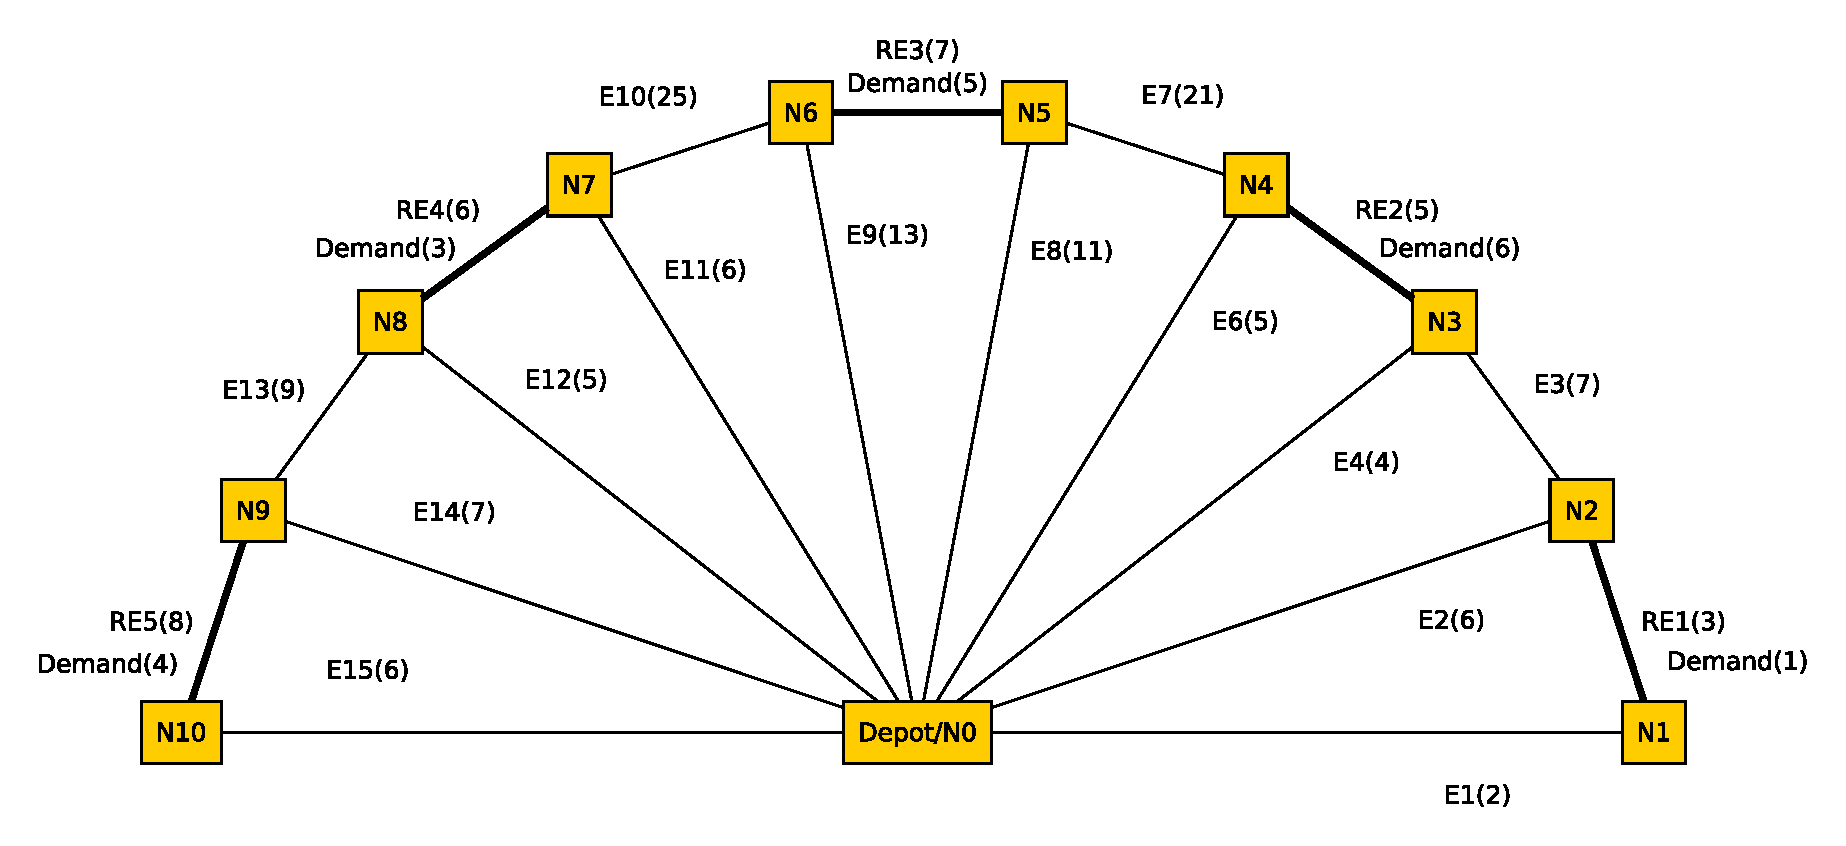
\includegraphics[width=\textwidth]{figures/SplitIllustrations/Split_GraphWithShortestPathsPlain.pdf}}
    \caption{Graph instance processed by the split algorithm. Edge traversal cost is given in the parentheses, and the required edges are marked with bold. The vehicle demand capacity is 8.}
    \label{fig:sgwspp}
\end{figure}

% \begin{algorithm}[thbp]
% \caption{Split}\label{split-pseudocode}
% \begin{algorithmic}[1]

% \Procedure{Split}{Genotype,Graph,Distances}
%     \State \textbf{let} $numberOfElements \leftarrow \sum (|N|+|E|+|A|) \in Graph$
%     \State \textbf{let} $e_k$ be the k'th element from the Genotypes ordering of the set $(N \cup E \cup A) \in Graph$ in its genome
%     \State \textbf{let} $costs$ be an array of length $numberOfElements + 1$
%     \State \textbf{let} $predecessors$ be an array of length $numberOfElements + 1$
%     \State \textbf{set} all entries in $costs$ to $\infty$
%     \State $costs[0] \leftarrow 0$
%     \State $predecessors[0] \leftarrow 0$
%     \Statex
%     \For{$i \leftarrow 1$ \textbf{to} $numberOfElements + 1$}
%         \State $j \leftarrow i$
%         \State $load \leftarrow 0$
%         \State $cost \leftarrow 0$
%         \DoWhile
%             \State $load \leftarrow load + e_j.demand$
%             \Statex
%             \If{$i = j$}
%                 \State $cost \leftarrow($ distance from depot to $e_{i-1}) + e_{i-1}.servicing\_cost +($ distance from $e_{i-1}$ to the depot $)$
%             \Else
%                 \State $cost \leftarrow  cost - ($ distance from $e_{j-2}$ to depot $) + ($distance from $e_{j-2}$ to $e_{j-1}) + e_{j-1}.servicing\_cost +($ distance from $e_{j-1}$ to the depot $)$
%             \EndIf
%             \Statex
%             \If{$(load < vehicle\_capacity)\wedge(costs[i - 1] + cost < costs[j])$}
%                 \State $costs[j] \leftarrow costs[i - 1] + cost$
%                 \State $predecessors[j] \leftarrow i - 1$
%             \EndIf
%             \Statex
%             \State $j \leftarrow j + 1$
%         \EndDoWhile{$(j < numberOfElements + 1)\wedge(load < vehicle\_capacity)$}
%     \EndFor
%     \Statex
%     \State \textbf{let} $Genotype.fitness \leftarrow costs[last\_index]$
% \EndProcedure

% \end{algorithmic}
% \end{algorithm}

The way the algorithm works to find the sub-trip of least cost that services the current element is as follows. For each required element in the supplied trip, it checks whether going from the depot, servicing the element, and going back is the least cost sub-trip. If so, the algorithm updates the list of predecessors indicating that going straight to the element from the depot is the best sub-trip for servicing it. At the same time, the elements value in the array of least costs of going to each element in the sub-trips is updated. The new value becomes the sum of the shortest paths of the previous splitted sub-trips, plus the new found cost of visiting this element in its own sub-trip.

\begin{figure}[thbp]
    \centerline{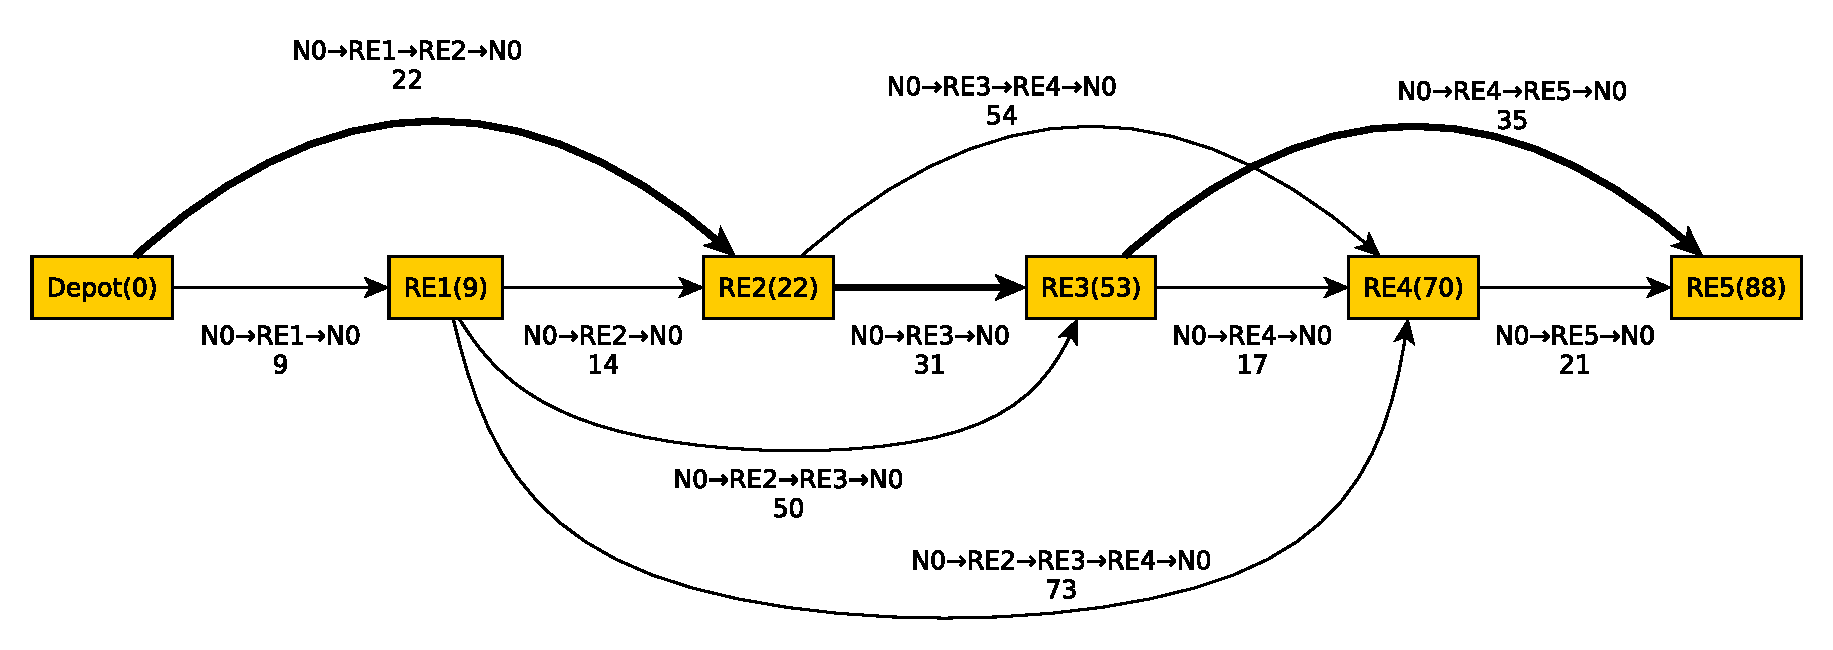
\includegraphics[width=\textwidth]{figures/SplitIllustrations/Split_AuxiliaryGraph.pdf}}
    \caption{The auxiliary graph built by split to process the graph shown in Figure \ref{fig:sgwspp}. The least cost of processing each required edge found is shown in parentheses in their respective nodes in the auxiliary graph. The least-cost path through all required elements is highlighted with bold arrows.}
    \label{fig:sag}
\end{figure}

After this, the algorithm tries to add one and one more required element to the current splitted sub-trip, until the next added element would exceed the vehicles capacity for servicing demand. To do the check, the algorithm first removes the cost of going from the last element in the currently splitted trip back to the depot from the end of the trip. Then the cost of going to the next required element, and from that element to the depot, is added to the cost. If this updated cost is lower than the currently lowest known cost for reaching the next element, and the demand load is manageable, the costs and predecessors arrays are updated. The next elements cost in the costs array is updated to the current cost, and its entry in the predecessors array is set to the index of the node at the beginning of the sub-trip currently being considered.

This process of adding an element at a time to existing or new trips and checking whether the sum of demand is permissible and the length of the trip can be taught of as generating an auxiliary graph. If one uses the graph in Figure \ref{fig:sgwspp} as an example, the resulting auxiliary graph would be the one shown in Figure \ref{fig:sag}.

For the purposes of finding the fitness value, the algorithm makes it as simple as looking at the last entry in the costs array. It is the sum of the costs of the shortest possible sub-trips leading up to the sub-trip containing the last element. Because the cost of this sub-trip also contains the last element and its cost, it is the cost of traversing all the sub-trips.

\begin{figure}[thbp]
    \centerline{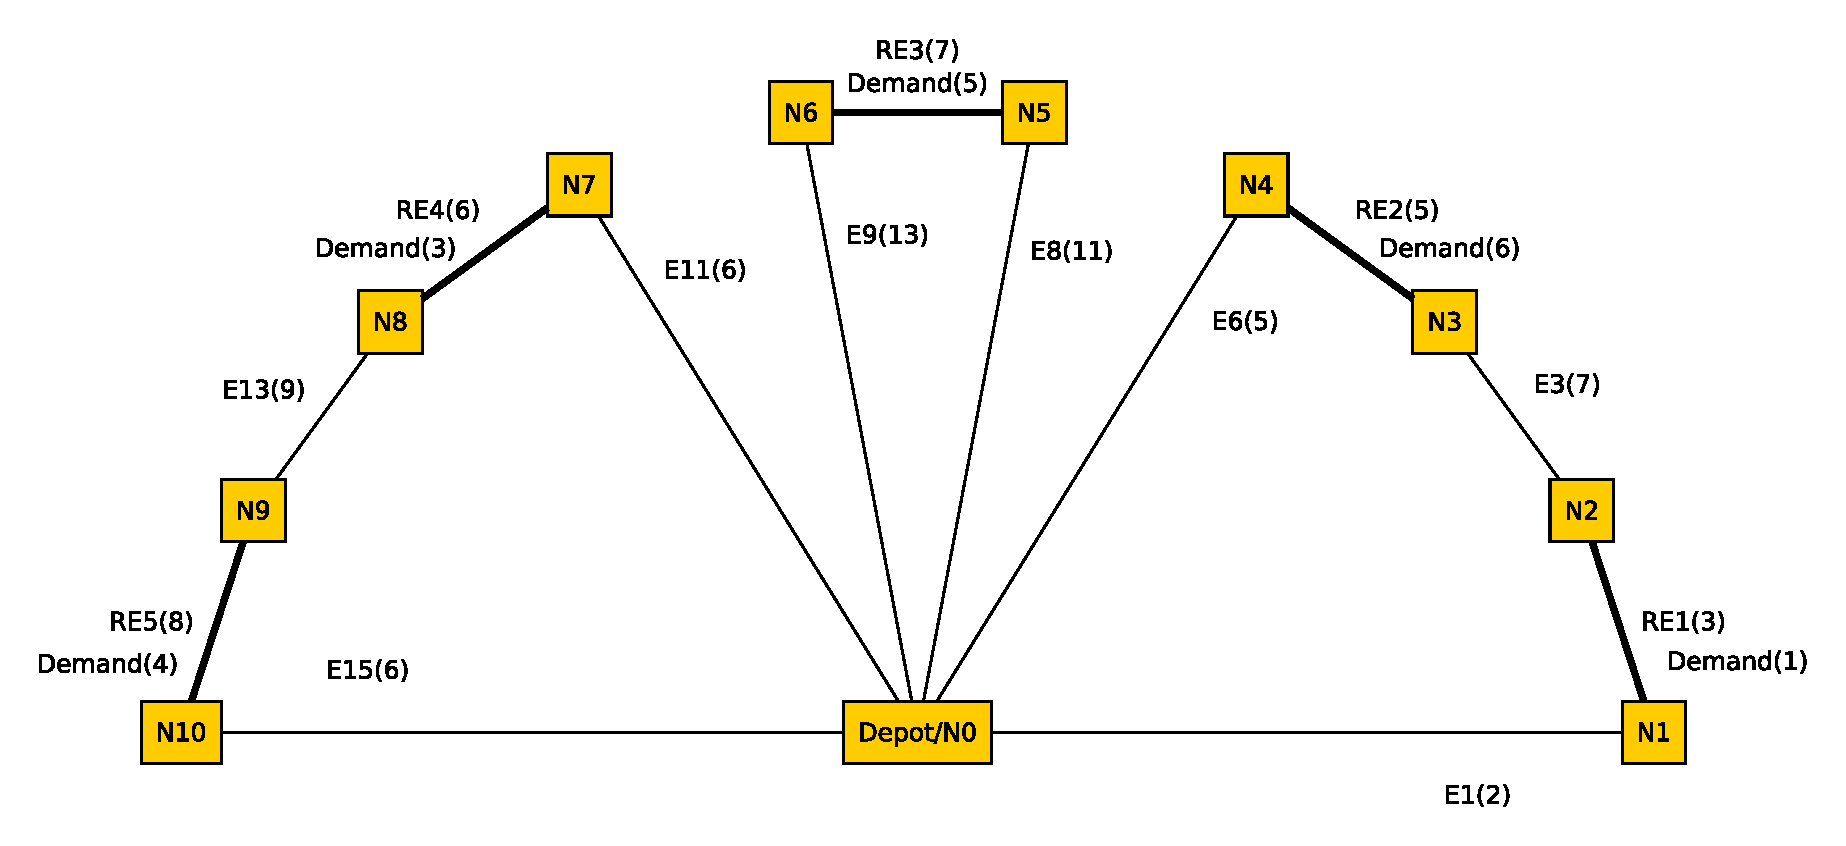
\includegraphics[width=\textwidth]{figures/SplitIllustrations/Split_GraphWithRoutes.pdf}}
    \caption{The trips generated from processing the graph in Figure \ref{fig:sgwspp} with the split algorithm.}
    \label{fig:sgwr}
\end{figure}

The retrieval of the resulting trips is shown in Algorithm \ref{split-retrieve-pseudocode} in Appendix \ref{sec:split_retrieve_trips_pseudocode}. This algorithm works by starting with the last node of the last splitted sub-trip and iterating over the predecessor array gotten from the Split algorithm. That gives it a worst case running time of $O(|\text{required elements}|)$. However, that is still less than the asymptotical worst case of the split algorithm that is $O(|\text{required elements}|^2)$. An example of trips that would be retrieved from the graph Figure \ref{fig:sgwspp} illustrates is shown in Figure \ref{fig:sgwr}.

% \begin{algorithm}[thbp]
% \caption{Retrieve Trips from Split}\label{split-retrieve-pseudocode}
% \begin{algorithmic}[1]

% \Procedure{Retrieve Trips From Split}{predecessors, genotype}
%     \State \textbf{let} $list\_of\_trips$ be an empty list
%     \State $j \leftarrow$ number of tasks
%     \DoWhile
%         \State $i \leftarrow predecessors[j]$
%         \State \textbf{let} $current\_trip$ be a new array of size $j - i$
%         \For{$k \leftarrow i + 1$ \textbf{to} $k \leq j$, $k \leftarrow k + 1$}
%             \State $current\_trip[k-(i+1)] \leftarrow genotype.genome[k-1]$
%         \EndFor
%         \State \textbf{add} $current\_trip$ \textbf{to} the beginning of $list\_of\_trips$
%         \State $j \leftarrow i$
%     \EndDoWhile{$i \neq 0$}
% \EndProcedure

% \end{algorithmic}
% \end{algorithm}


% subsection the_split_algorithm (end)
% section evolutionary_algorithms (end)
% chapter theory (end)

\cleardoublepage
